\documentclass[a4paper,12pt]{article} 

%paquetes
\usepackage{graphicx}
\usepackage[spanish]{babel} 
\usepackage[utf8]{inputenc}
\usepackage{textcomp}
\usepackage{float}
\usepackage{subfig}
\usepackage{listings}

%caracteristicas de paginas
\pdfpagewidth 8.5in
\pdfpageheight 11in
\setlength\oddsidemargin{-0,21in}
\setlength\evensidemargin{-0,21in}
\setlength\topmargin{-2cm}
\setlength\textwidth{7in}
\setlength\textheight{9in}
\setlength\parskip{0.1in}

%%%%%%%%%%%%%%%%%%%%%%%%%%%%%%%%%%%%%%%%%%%%%%%%%%%%%%%%%%%%%

\begin{document} 

\title{Introducci\'on a la soluci\'on num\'erica de ODE's \\
\large Gu\'ia computacional 1 - Mec\'anica Cl\'asica 2016 - Clase G. Mindlin}
\author{Ignacio Poggi - L.U: 567/07 - ignaciop.3@gmail.com}
\maketitle

%\tableofcontents  %lo ponemos para trabajo largos que necesiten indice


\section{Enunciado}

En la secci\'on de materiales adicionales de la c\'atedra se encuentra un programa principal y un integrador Runge-Kutta de orden 4 (rk4) en lenguaje C. En el programa principal se encuentra escrita una ecuaci\'on diferencial a integrar, los par\'ametros y las condiciones iniciales. Sobre este c\'odigo van a trabajar en las siguientes actividades realizando las modificaciones pertinentes para su problema en particular.

En ubuntu es posible compilar y ejecutar el c\'odigo directamente desde una terminal abierta en una carpeta que contenga tanto el programa principal como el integrador rk4:\newline

\framebox[1.1\width]{gcc ODE\_ejX.c -o ode\_ejX -lm rk4.c}

\framebox[1.1\width]{./ode\_ejX}\newline

Se obtendr\'a como salida un archivo llamado $ejX.dat$ , donde $X$ es el n\'umero del ejercicio, que contiene el resultado de la integraci\'on. Los resultados pueden ser analizados graficamente mediante un graficador, en nuestro caso utilizaremos \textbf{gnuplot} que se controla mediante comandos en terminal.\newline


{\Large \textbf{Actividad 1}}

Editar el codigo de ODE.c para analizar los siguientes puntos:

\begin{itemize}
\item C\'omo var\'ia el resultado seg\'un el paso de integraci\'on. Programe una integraci\'on con el m\'etodo de Euler y compare.
\item Analizar c\'omo evoluciona el sistema dadas distintas condiciones iniciales.
\end{itemize}
Qu\'e tipo de conclusiones puede obtener a partir de los an\'alisis anteriormente realizados.\newline


{\Large \textbf{Actividad 2 - Oscilador arm\'onico amortiguado}}

El oscilador arm\'onico amotiguado es un problema del cual se conoce la soluci\'on anal\'itica cuya ecuaci\'on diferencial que rige el movimiento es:

\begin{equation}
	\frac{d^2 x}{dt^2} + 2\gamma\frac{dx}{dt} + \omega_0^2x = 0
\end{equation}

Estudie num\'ericamente las soluciones del sistema seg\'un la relaci\'on de los par\'ametros, para ello: escriba la ecuaci\'on de segundo orden como dos ecuaciones de primer orden, var\'ie $\gamma$ y $\omega$ e integre. Tambi\'en analice distintas condiciones iniciales. Compare con lo conocido de la soluci\'on anal\'itica, para ello grafique como evoluciona la posici\'on en el tiempo, la velocidad y cu\'al es la trayectoria en el espacio de fases $x  \ddot{x}$.\newline


{\Large \textbf{Actividad 3 - Oscilador de Van der Pol}}

Es un tipo de oscilador con un amortiguamiento no lineal descripto a principio de siglo por Van der Pol quien estudi\'o circuitos el\'ectricos con componenten no lineales obteniendo la ecuaci\'on:

\begin{equation}
	\frac{d^2 x}{dt^2} + \mu(x^2-1)\frac{dx}{dt} + x = 0
\end{equation}

Este sistema presenta soluciones oscilatorias para ciertos valores del par\'ametro $\mu$ que son conocidad como oscilaciones de relajaci\'on. Esta ecuaci\'on tiene una importancia en la ciencia ya que fue usada en distintos campos para describir por ejemplo, el comportamiento de una falla tect\'onica o el potencial de acci\'on de una neurona. Esto se debe a que el sistema seg\'un los valores de $x$ presenta un amortiguamiento positivo (como el de la actividad 2 donde el sistema pierde energ\'ia), y para otros presenta un amortiguamiento "negativo" donde el sistema gana energ\'ia. Esto produce que eventualmente la energ\'ia perdida en un ciclo sea igual a la ganada generando oscilaciones autosostenidas. Este sistema se ver\'a con m\'as detalle avanzado el curso, en esta pr\'actica se propone realizar un acercamiento de forma num\'erica para tener cierta comprensi\'on de c\'omo se comporta el mismo.

\begin{itemize}
\item Escriba el sistema como dos ecuaciones de primer orden.
\item Inspecione num\'ericamente las soluciones posibles del sistema, estudie como var\'ian seg\'un la variaci\'on del par\'ametro $\mu$. Para ello grafique la trayectoria $x$ en funci\'on del tiempo, la velocidad $\ddot{x}$ en funci\'on del tiempo y tambi\'en el espacio de fases $x  \ddot{x}$.
\item Modifique tambi\'en las condiciones iniciales y estudie num\'ericamente las respuestas del sistema. Para ello grafique la trayectoria $x$ en funci\'on del tiempo, la velocidad $\ddot{x}$ en funci\'on del tiempo y tambi\'en el espacio de fases $x  \ddot{x}$.
\end{itemize}


{\Large \textbf{A entregar}}

Se deber\'a entregar un trabajo de la actividad 2 y 3, con los c\'odigos, los gr\'aficos obtenidos para las integraciones num\'ericas propuestas y el correspondiente an\'alisis para cada caso.



\begin{figure}[H]
\begin{center}
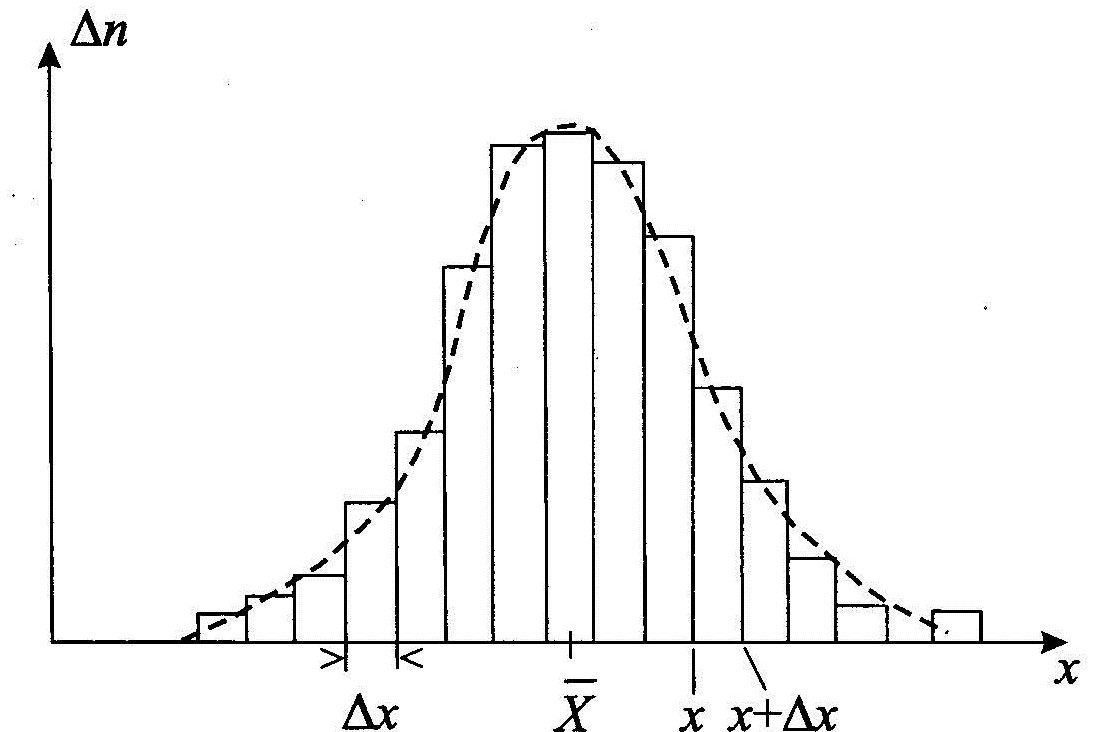
\includegraphics[height=8cm]{histograma.JPG}
\caption[width=5cm]{Histograma}
\label{hcongauss}
\end{center}
\end{figure}




\section{An\'alisis de datos y conclusiones}
\subsection{Oscilador arm\'onico amortiguado}

Para su desarrollo se requirieron de los siguientes materiales:
\begin{itemize}\item Soporte de 1.5 metros de altura
\item Sensor optico (photogate)
\item Hilo inextensible
\item Bolita metálica
\item Fósforo
\item Cinta métrica (apreciación 0,001 m)
\item Software (Precission Timer, Origin 6.0)
\end{itemize}

Previo al montaje del experimento fue necesario medir de forma directa las magnitudes fisicas formalmente involucradas.

Masa del sistema: 112,00 g

Radio de la esfera: 30, 2 mm

Longitud del fósforo: 40 mm

Largo de la cabeza del tornillo: 9,22 mm


Una vez medidas, para el armado del modelo unimos un fósforo a una bolita metálica de manera que el photogate pueda captar la oscilación con exactitud. Se sujeto la bolita a un extremo del hilo y el otro extremo se fijo al soporte. De manera que el dispositivo sea semejante al de la figura (\ref{figpendulo})

 \begin{figure}[H]
\begin{center}
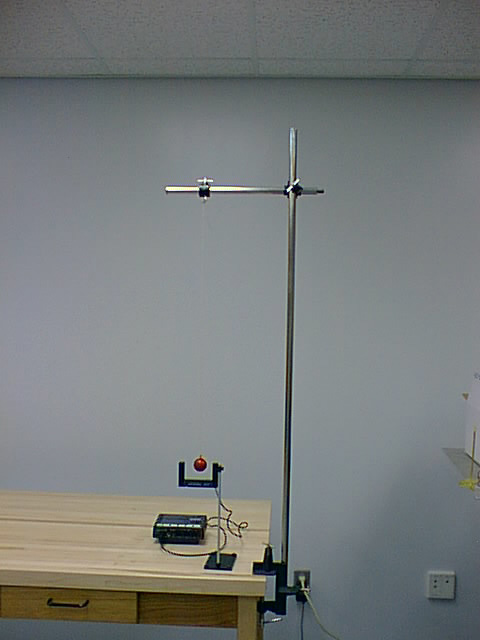
\includegraphics[height=10cm]{SimplePendulum.jpg}
\caption[width=5cm]{Sistema del pendulo armado con la esfera colocada de tal forma que el fosforo adherido a la esfera bloquee el haz de luz al pasar}
\label{figpendulo}
\end{center}
\end{figure}




Al tomar la aproximacion de peque\~nas oscilaciones, el ángulo de desviación máximo respecto a la vertical fue de 10\textdegree. La longitud fue tomada con cinta métrica (desde el punto de suspensión hasta el centro de la cabeza del tornillo,a lo que se le sumo la altura de la cabeza del tornillo y el radio de la esfera), de manera de tener la longitud desde el punto de vinculo al centro de masa. Una vez montado el dispositivo se procede a adecuar el hilo a la longitud deseada. Luego se aparta la esfera de la vertical, y se la deja oscilar libremente. Se midio el período de 3 series de 50 oscilaciones del pendulo para 10 longitudes distintas (desde 0,60m a 1,50 m con intervalos de 0,1 m) utilizando el photogate y los equipos de adquisición de datos con el programa Precision Timer.


\subsection{Oscilador de Van der Pol}

A partir de las 50 mediciones del periodo del pendulo hechas en cada serie a distintas longitudes, se calcul\'o su valor medio.

Es importante aclarar que obtenidos los valores medios fue necesario conocer la desviaci\'on de cada uno de ellos. Para lo cual aplicamos la siguiente f\'ormula:

\begin{equation}
 {\Delta y}^2=\sum\limits_{k=1}^n \left(\frac{\partial \textit{f}}{\partial x_{i}}  {(x_{1},x_{2},\ldots,x_{n})}\ldotp \Delta x_{i} \right)^2
\caption{F\'ormula de propagaci\'on de errores}
\label{propaerrores}
\end{equation}

$\Delta {T}$ fue obtenido a partir del software Origin. Mientras que para $\Delta {L}$ tuvimos que aplicar la f\'ormula (\ref{propaerrores}) ya que la medici\'on del punto de v\'inculo al centro de masa lo hicimos tomando las longitudes del hilo, la cabeza del tornillo y el redio de la esfera.


A partir de los datos obtenidos en la tabla (\ref{tabpromedios}) de forma directa, se realiz\'o un test de hip\'otesis estad\'istico. Es decir, determinar si los valores corresponden a una distribuci\'on gaussiana. Para ello, tomamos diferentes mediciones del periodo a distintas longitudes y graficamos la informaci\'on recolectada mediante histogramas. Con esta informaci\'on se procedi\'o a un ajuste Gaussiano



He aqui las distintas situaciones.


\section{Ap\'endice}

Descargar el archivo $guia1\_poggi.zip$ y descomprimirlo en una carpeta a elecci\'on del usuario, abrir una terminal dentro de la carpeta $\sim \backslash mecanica-clasica\backslash practica1$; y seguir las instrucciones provistas en la secci\'on Enunciado.

Los archivos que contienen los datos num\'ericos $(ej2.dat$ y $ej3.dat)$ no fueron transcriptos en este informe dada la extensi\'on de los mismos


\subsection{C\'odigo fuente en C del oscilador arm\'onico amortiguado (ODE\_ej2.c)}

\lstinputlisting[language=C,breaklines]{../ODE_ej2.c}

\subsection{C\'odigo fuente en C del oscilador de Van der Pol (ODE\_ej3.c)}
aasdasdjkasdjk

\subsection{C\'odigo fuente en C del m\'etodo de Runge-Kutta de orden 4 provisto por la c\'atedra (rk4.c)}
\lstinputlisting[language=C,breaklines]{../rk4.c}

\section{Bibliograf\'ia}




\end{document}
